% !TEX program = xelatex
\documentclass[sigconf,nonacm,anonymous,review]{acmart}

\usepackage{kotex}
\usepackage{graphicx}
\usepackage{booktabs}
\usepackage{array}
\usepackage{enumitem}
\usepackage{balance}
\usepackage{amsmath}
\usepackage{amssymb}
\usepackage{newunicodechar}
\usepackage{dblfloatfix}
\setlist[itemize]{leftmargin=*,nosep}
\settopmatter{printacmref=false, printccs=false, printfolios=true}
\renewcommand\footnotetextcopyrightpermission[1]{}
\pagestyle{plain}

% ---- unicode symbols used in the Korean body (xelatex) ----
\newunicodechar{→}{\ensuremath{\rightarrow}}
\newunicodechar{↔}{\ensuremath{\leftrightarrow}}
\newunicodechar{≤}{\ensuremath{\le}}
\newunicodechar{≥}{\ensuremath{\ge}}
\newunicodechar{≈}{\ensuremath{\approx}}
\newunicodechar{×}{\ensuremath{\times}}
\newunicodechar{∈}{\ensuremath{\in}}
\newunicodechar{±}{\ensuremath{\pm}}
\newunicodechar{·}{\textperiodcentered}
\newunicodechar{°}{\textdegree}
\newunicodechar{τ}{\ensuremath{\tau}}
\newunicodechar{✓}{\ensuremath{\checkmark}}
\newunicodechar{✗}{\ensuremath{\times}}
\newunicodechar{⓪}{(0)}
\newunicodechar{①}{(1)}
\newunicodechar{②}{(2)}
\newunicodechar{③}{(3)}
\newunicodechar{④}{(4)}
\newunicodechar{⑤}{(5)}
\newunicodechar{⑥}{(6)}
\newunicodechar{⑦}{(7)}

% placeholder box for figures whose plots are deferred this round
\newcommand{\figtodo}[1]{\fbox{\parbox[c][2.6cm][c]{.92\linewidth}{\centering\itshape #1\\[3pt]\normalfont\footnotesize[\,placeholder: plot inserted once measurements are in\,]}}}

\title{OVLA: On-device Verification of LLM-Generated IoT Automations via Timeline IR}
\author{Anonymous Submission}
\affiliation{\institution{Submitted to SenSys 2027}\country{}}
\email{}

\begin{document}

\begin{abstract}
Smart home automation increasingly relies on Large Language Models (LLMs) to translate natural language (NL) user intents into executable reactive rules. However, deploying these rules directly on edge hubs poses severe reliability and safety risks since reactive IoT automations are temporally complex, involving precise triggers, durations, and repetitions. Existing validation methods rely heavily on human code inspection, offline experts, or resource-heavy cloud LLM re-checks, failing edge privacy and latency constraints. To tackle this challenge, we present OVLA, an on-device pipeline for deterministic, LLM-free verification of IoT automations before deployment. OVLA bridges the gap between informal natural language and strict execution using Timeline IR, a compact, machine-checkable representation of temporal behavior. The pipeline first translates the user's NL intent into a typed Timeline IR; the user confirms a deterministic plain-language rendering of this IR, which then serves as the reference specification of the intended behavior. OVLA then automatically synthesizes reference event traces and boundary cases from this IR. An efficient verifier simulates the generated rule code against these traces to detect behavioral discrepancies and guide automated repairs via counterexamples. Evaluated with a local, quantized ≤9B model across 382 automations, OVLA caught every faulty program in our evaluation set, repairing 33\% of them and rejecting the rest fail-closed. Under 1,567 injected temporal bugs, it detected 99.3\%, while its synthesized scenarios exercised 97.4\% of specification-side obligations and 96.8\% of generated-code branches, raising the share of correctly deployed automations from 91.4\% to 94.2\%, all without any LLM in the verification loop.
\end{abstract}

\keywords{IoT automation, LLM code generation, reactive-temporal code, deterministic verification, on-device, trace equivalence}

\maketitle

\section{Introduction}

IoT automation is rapidly moving toward LLM-based code generation. A user states the desired behavior in natural language, and an LLM turns it into a reactive rule the platform can execute. Yet the final step of this workflow, deciding \emph{whether the generated code is correct to deploy}, has no deterministic gate. The missing piece is a reference to check the code against; the natural-language request contains the intent, but not in a form that can serve as a rigorous baseline for automated testing.

\textbf{Why this is hard: %there is nothing to check against.
} The core challenge stems from the absence of a verifiable reference baseline. The target automations are inherently \emph{reactive-temporal}. They are \emph{reactive} because their execution is driven by asynchronous events and conditional triggers, % (triggers, waits on conditions), 
and \emph{temporal} because their behavior unfolds over time through schedules, periodic executions, and sustained state durations (e.g. ``if it persists for more than N minutes'').
%it is also driven by time (schedules, periodic execution, sustained durations such as ``if it persists for more than N minutes''). With 
Driven by timers, counters, and multi-step state, the correct behavior of an automation must be evaluated across an entire timeline rather than a single discrete instant. Furthermore, in our setting, this logic is deployed as arbitrary code rather than a restricted, fixed-rule template.
%the behavior is defined over a timeline rather than at a single instant, and in our setting it is deployed as \emph{code}, not as a fixed rule template. 
%Two properties make deciding their correctness hard. 
Validating their correctness presents two key challenges. First, no test oracle is available. 
Unlike text-to-SQL or traditional programming benchmarks that supply gold denotations or input-output test suites, a reactive automation's output is a future sequence of environment interactions. Because no external source can pre-label this sequence, the verification reference must be actively constructed on the fly. 
%The intended behavior is fixed by the user's request, but nothing provides it as a checkable artifact: the request was given moments ago, it may admit more than one valid realization, and no benchmark supplies a gold answer. Unlike text-to-SQL, whose benchmarks supply a gold denotation, or algorithmic code, which ships with input-output tests, a reactive automation's output is a future sequence of device actions that no external source labels as correct, so the reference has to be constructed rather than looked up. Second, the same intended behavior admits many syntactically different yet behaviorally equivalent realizations,
Second, syntactic divergence complicates evaluation. The same user intent can be expressed through many syntactically different yet behaviorally equivalent implementations. Therefore, checking a generated program by matching it against any single reference text is neither sound nor complete. Determining correctness fundamentally requires reasoning about the program’s semantic behavior over time, rather than analyzing its static syntax or a single snapshot of its output. %Deciding whether the code is correct therefore means reasoning about its behavior over time, not about its syntax or a single output.

\textbf{Running example:} Suppose a user requests ``whenever the temperature rises above 25°C, turn on the air conditioner.'' We read ``rises above'' as an edge-triggered intent: the AC should be switched on once per upward crossing, not continuously while it stays hot. Figure~\ref{fig:idiom} shows three lowerings, sketched in JoI, the automation DSL of our target platform (\S4). Implementation (a) detects the crossing by comparing the previous and current temperature readings while (b) keeps a flag that is set on firing and reset when the temperature falls back below the threshold. (a) and (b) share almost nothing syntactically yet behave identically, so no syntactic comparison can certify one against the other. Implementation (c) appears to be the most intuitive translation %natural-looking lowering
because it textually mirrors the natural-language request. However, %reads like the request itself, and 
it is the wrong one: under periodic execution it falsely re-fires on every tick as long as the temperature stays above the threshold. All three are syntactically valid and look plausible; they can only be differentiated by evaluating their execution traces over time; %only the action traces separate them, and 
because repeated On() commands leave the AC in the same visible state, the user may see nothing wrong. This is a crucial failure mode our system eliminates: \textbf{deployed code that silently diverges from the user's intended behavioral specification}. (In the sketches, \texttt{cron} sets when the script starts, \texttt{period} is the tick interval in milliseconds, and \texttt{code} is the body executed on every tick; \texttt{:=} initializes a persistent variable once, while \texttt{=} performs per-tick update.) %updates it per tick.)

\begin{figure}[t]
\centering

\includegraphics[width=\linewidth]{figs/figure1_a.pdf}\par
{\small (a) Previous/current comparison}\par\smallskip
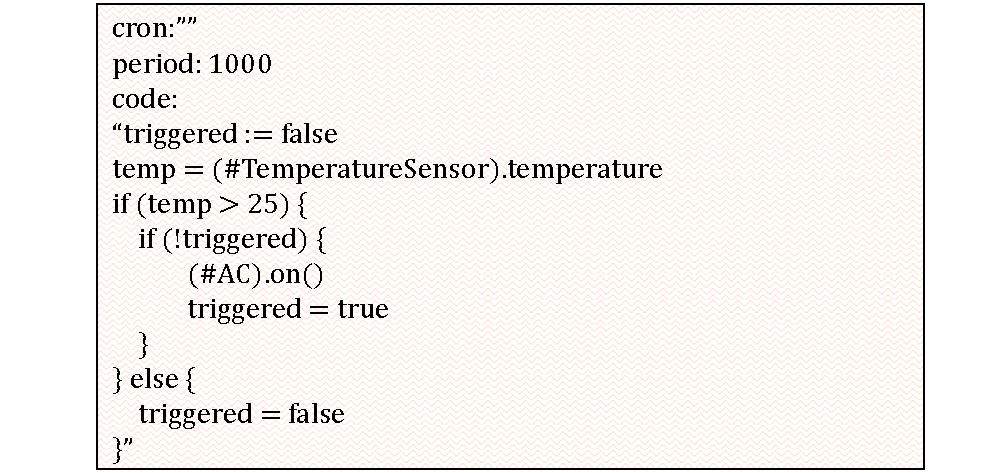
\includegraphics[width=\linewidth]{figs/figure1_b.pdf}\par
{\small (b) Triggered flag}\par\smallskip

\includegraphics[width=\linewidth]{figs/figure1_c.pdf}\par
{\small (c) Re-fires while the level holds}\par\smallskip
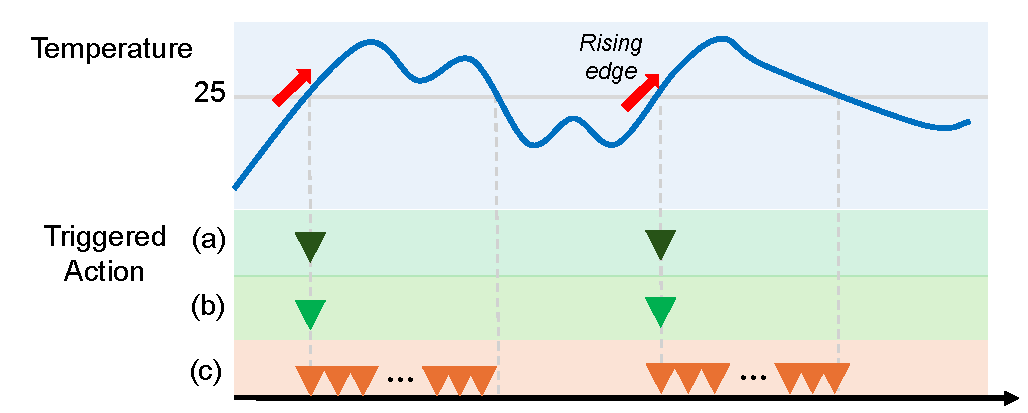
\includegraphics[width=\linewidth]{figs/figure1_trace.pdf}\par
{\small (d) Action traces}
\caption{Three lowering sketches of one intent (``whenever the temperature rises above 25°C, turn on the air conditioner'') and their action traces. (a) and (b) produce identical traces; (c) fires on every tick while the threshold is exceeded.}
\label{fig:idiom}
\end{figure}

\textbf{Why existing checks fall short.} %do not close the gap.} 
Prior verification frameworks of IoT automations target fixed, predefined criteria rather than the user's intent. A large body of work checks hand-authored trigger-action rules; for instance model checkers prove safety properties, inter-rule conflicts, or security policies (e.g., AutoTap~\cite{autotap}), while runtime monitors flag deviations from mined invariants~\cite{hawatcher}. This limitation is a consequence of design paradigm, not oversight. When a user writes the rule directly, the rule itself serves as %\emph{is} 
the ground-truth intent, and critical risks worth verifying, such as rule conflicts and security violations, can be defined, without referencing the unique intended behavior of a specific task. % are defined without reference to any one task's intended behavior. 
However, as the user transitions from author to prompter, the verification paradigm fundamentally changes. Once an LLM synthesizes code from a natural-language request, the user’s original statement and the generated artifact become distinct, decoupled entities that can silently diverge. In this generative workflow intent-conformance emerge as a critical, unaddressed checkpoint.
%When the user stops being the author, the question changes: once an LLM writes the code from a natural-language request, what the user said and what was produced become two separate artifacts that can disagree, and only then does intent-conformance become a question to check.

In that generation setting, the gap remains wide open, and bridging it hinges on a single question: %real but unfilled, and whether a system closes it turns on one question: 
does a test oracle already exist? Generators designed for algorithmic IoT code can readily validate their output against executable test suites or labeled accuracy, similar to how text-to-SQL frameworks verify relational denotations. For these domains, intent-conformance is effectively a solved problem (e.g., GPIoT~\cite{gpiot}). Reactive automations, however, lack any such ready-made oracle. Hence natural language-to-automation generators must settle for weaker proxies: schema validity (e.g., verifying that the framework accepts the JSON syntax), device grounding feasibility, lexical matching against ground-truth commands, or evaluation by an LLM judge. Even frameworks that present the generated rule back to the user rely on manual, error-prone human-in-the-loop confirmation rather than formal verification of the underlying executable code (e.g., AwareAuto [16]). To date, no existing system deterministically verifies that reactive-temporal code faithfully executes the user's behavioral intent over time. The fundamental missing piece is not a more capable language model, but a verifiable reference specification. %schema validity (the framework accepts the JSON), grounding feasibility, ground-truth command matching, or an LLM judge; and even those that show the generated rule back to the user have the user confirm it by hand rather than checking the code against it (AwareAuto~\cite{awareauto}). None checks deterministically that reactive-temporal code behaves as intended. The missing piece is not a better model but a reference to check against.

\textbf{Why not an LLM judge.} The remaining alternative that targets user intent directly is to ask another LLM whether the code matches the request. But an LLM judge is too unstable to act as a deployment gate. A deployment decision is binary: two behaviorally identical programs must receive the same deploy/reject verdict. Yet we find that on behavior-preserving programs that differ only in idiom, an LLM judge's verdict flips even at temperature 0 (\S3). Larger models still flip, and cloud models violate the privacy and latency constraints of the edge. A gate whose verdict tracks the surface form of the code is not fit to gate deployment.

\textbf{OVLA.} To address these challenges, we present OVLA. Its key idea is to \emph{derive the missing reference specification} at authoring time and subsequently utilize it as a deterministic verification baseline. %check against it deterministically. 
First, OVLA builds a candidate Timeline IR from a natural-language request. Then, the system generates a deterministic, plain-language Rendering of this IR for the user to review and confirm. % , ; the user confirms its deterministic plain-language Rendering; and 
This confirmed IR serves as a per-automation behavioral oracle. The generated JoI code is then verified against the oracle by bounded trace-equivalence over the finite set of transition points defined by the IR. Both components are run on events synthesized at those points (e.g., timer expirations, condition thresholds, and cycle restarts), and their resulting action traces are compared. While the LLM is confined to \emph{generation}, proposing the IR and lowering it to code, both the rendering step and the equivalence check are deterministic and LLM-free. This allows conformant automations to be safely deployed at the edge without cloud-side review. \emph{Precisely because} lowering relies on a probabilistic LLM, %is an LLM stage, 
a deterministic checker is needed.

\textbf{Scope and assumptions.} 
OVLA targets natural-language commands specifying explicit reactive-temporal behaviors. Inferring intent from vague or affective goals (e.g., "make it cozy") is a separate intent-elicitation challenge addressed by orthogonal literature (e.g., Sasha~\cite{sasha}, SAGE~\cite{sage}) and is strictly out of scope. Any residual ambiguity within a specifiable command is intentionally surfaced by OVLA's deterministic Rendering phase and resolved during user confirmation, rather than by the verifier itself. 
%OVLA's input is a natural-language command that names a specific reactive-temporal behavior. Inferring what behavior a user would want from an affective or underspecified goal (``make it cozy'') is a separate intent-elicitation problem (Sasha~\cite{sasha}, SAGE~\cite{sage}) and is out of scope; residual ambiguity in a specifiable command is surfaced by the deterministic Rendering and resolved at confirmation, not by the verifier. 
Confirming the IR is presented as a plain-language judgment rather than a programming task. The dimensions a user controls in reactive-temporal automation are limited and enumerable (start time, period, trigger and condition, action and its arguments, sustain and delay durations), Timeline IR expresses only these slots, and deterministic Rendering displays them verbatim as a readable timeline (\S8.3). Approving an IR is thus a closed judgment over finite control slots the command named, not the authoring of arbitrary formal properties.

\textbf{Two-layer guarantee.} We explicitly define the boundaries of our verification scope. %We are explicit about how far the guarantee reaches. 
In \textbf{Layer A (NL→IR)}, the system captures intent as IR and presents it in plain language, but we do not measure non-expert confirmation success \emph{itself} in this round via a human-subjects study (\S9). In \textbf{Layer B (IR→code)}, once the IR is approved, OVLA prevents the generated code from silently diverging from that displayed IR within a bounded behavior region. OVLA's technical guarantee lies firmly in Layer B.

\textbf{Deployment setting.} We assume a home edge device rather than the cloud, to ensure privacy (sensor data never leaves the home) and reduce latency. %for privacy (sensor data never leaves the home) and latency. 
This environment precludes a cloud LLM judge, requiring the validation gate to be an LLM-free deterministic check. Consequently, a single design decision simultaneously delivers trust (via a non-probabilistic judge) and deployability (millisecond-level localized execution with zero model-call overhead).
%This constraint excludes a cloud LLM judge from the gate, so the gate must be an LLM-free deterministic check. A single design decision yields both trust (no probabilistic judge) and deployability (milliseconds, no model call).

\medskip\noindent\textbf{Contributions.} 
To the best of our knowledge, OVLA is the first system for LLM-generated reactive-temporal IoT automations that transforms intent-conformance into a deterministic, pre-deployment verification check. It achieves this by establishing a user-confirmed behavioral IR as the authoritative test oracle, rather than relying on a probabilistic judge or superficial manual review. %To our knowledge, OVLA is the first system for LLM-generated reactive-temporal IoT automations to turn intent-conformance into a deterministic pre-deployment check, using a user-confirmed behavioral IR as the oracle rather than a probabilistic judge or manual review.
\begin{itemize}
\item \textbf{C1. Timeline IR:} We introduce a unified representation that simultaneously serves dual roles: % A single representation plays two roles at once: 
(a) a surface that is deterministically rendered to plain language for user validation, and (b) a machine-checkable behavioral reference for validating reactive-temporal code. While an approved NL sentence can serve only (a) and a formal property only (b), our contribution lies in a singular representation that achieves both. Given that prior works can already generate confirmable temporal IRs, our distinct claim is the novel integration of deterministic, LLM-free verification, automatic rendering, and localized on-device operation %since prior work already generates confirmable temporal IR, our claim is the \emph{combination} of deterministic LLM-free verification, rendering, and on-device operation 
(\S2).
\item \textbf{C2. Deterministic deployment gate:} We propose an end-to-end pipeline, spanning IR→FSM→boundary event→bounded trace-equivalence, that executes entirely without LLM intervention. The gate operates under a fail-closed policy where a pass triggers immediate deployment and a failure triggers automatic repair or rejection. % (pass=deploy / fail=repair or reject). 
When the gate flags an anomaly, it guarantees a genuine behavioral divergence under the defined observation model, ensuring rejection-soundness.
\item \textbf{C3. On-device realization:} The generation phase utilizes a 4-bit quantized model of at most 9 billion parameters without any fine-tuning, while the verification gate bypasses LLM execution entirely. Consequently, verification completes locally in about a millisecond at the median. OVLA's verification guarantee does not depend on the size or quality of the generation model.
\item \textbf{C4. Evaluation:} We empirically demonstrate system safety by mitigating silent IR-to-code divergence from 8.6\% down to 0\% (\S8.1). Furthermore, we evaluate verifier detection accuracy (\S8.2), rendering faithfulness (\S8.3), and on-device execution overheads and deployment feasibility (\S8.4) through rigorous component-by-component analysis.
\end{itemize}

\textbf{Focus of the contribution.} OVLA removes a failure mode that survives user approval: even when the approved IR is acceptable, the subsequent reactive-temporal lowering phase can introduce subtle state, timer, and boundary errors that cause the deployed code to diverge. OVLA serves as the deterministic, on-device gate specifically engineered to intercept and remediate exactly these errors.

\section{Related Work and Positioning}

Verification of home automations did not begin as an open problem. When users authored rules directly, the rule itself was the artifact under analysis, and formal techniques could check it against fixed properties; when code was generated in domains that ship executable tests, the tests served as the oracle. In both settings, a checkable reference existed before verification began. LLMs entered this workflow for a practical reason: authoring is the bottleneck, as end users struggle to write and debug even slot-based rules, and richer reactive-temporal behaviors require code they cannot write at all. This shift turns the user from an author into a prompter, separates the request from the artifact that implements it, and removes the very reference that earlier verification relied on. We therefore organize prior work by the reference each system checks against.

\textbf{When a verification reference already exists.} A rich body of work verifies hand-authored TAP rules with formal techniques. AutoTap~\cite{autotap} synthesizes or repairs TAP rules, modeled as transition systems, so that they satisfy LTL safety property templates chosen by the user. TAPInspector~\cite{tapinspector} model-checks timing-aware rule sets for safety and liveness violations and TAPFixer~\cite{tapfixer} repairs such violations; related analyses uncover inter-rule and security vulnerabilities~\cite{iruler,soteria}; and HAWatcher~\cite{hawatcher} monitors deployed automations against mined invariants at runtime. Deterministic verification is possible in this line because the reference is fixed in advance: a safety property, conflict freedom, or a security policy. Because the user authors the rule directly, the rule is itself the artifact under analysis, and a separate per-task intent reference is never required.

The same holds for generation targets whose domain supplies an executable oracle. GPIoT~\cite{gpiot} generates signal-processing and ML algorithm code from natural-language requirements using an on-device fine-tuned SLM and verifies the result with pass@k execution tests. Outside IoT, text-to-SQL verifies a generated query against the denotation of a gold query~\cite{spider}, and CodeT~\cite{codet} and Self-Debug~\cite{selfdebug} verify generated code with unit tests. \emph{Across both lines, verification was enabled by a checkable target that was already available, whether a fixed property, a test suite, or a gold denotation.}

\textbf{LLM-generated reactive automations: no ready-made reference.} LLM-generated reactive automations have no such target: the intended behavior is named only in the user's request, and no benchmark or test suite labels its future action sequence. The missing reference is also harder to substitute here than for TAP rules. TAP rules do carry temporal behavior, including triggers, stays-for durations, and cron-style schedules, but there it is a platform \emph{primitive}: the author fills slots and the engine implements the mechanism, so slot errors are visible on the face of the rule. In reactive-temporal code such as JoI scripts, no such primitive exists for edge detection, sustained conditions, or counting; the author, here an LLM, must realize the mechanism as an \emph{idiom} built from persistent variables, conditions, and per-tick execution. Mechanism errors are silent, and they are exactly where lowering bugs arise.

Some systems in this regime do check LLM output deterministically, but still against fixed criteria. AutoIoT~\cite{autoiot_maude} checks LLM-generated rules against four inter-rule conflict types using Maude rewriting logic. DS-IA~\cite{dsia} checks the device-grounding feasibility of a command with a deterministic cascade and rejects infeasible commands fail-closed before execution. TaskSense~\cite{tasksense} translates a sensing query into an executable tool-calling DAG, screens it with an LLM-based solvability check, and then deterministically checks that the plan's dependency graph is a subgraph of the toolset grammar; both checks establish structural well-formedness, and its only behavioral reference, a hand-authored ground-truth plan, exists solely in offline evaluation. AgentSpec~\cite{agentspec} enforces trigger-predicate safety rules on LLM agents at runtime through a deterministic DSL; however, its rules are fixed and hand-written rather than derived from the request being served. \emph{Most of these checks are deterministic, yet their reference remains a predefined criterion; the behavior the user actually asked for is still never the reference.}

Generation systems themselves fall back to weaker checks. ChatIoT~\cite{chatiot} translates natural language into Home Assistant automations with multiple LLM agents and has a separate ``Evaluator'' agent assess format compliance and request satisfaction; Giudici et al.~\cite{giudici2025} accept a generated routine if the framework parses its JSON; and IoTGPT~\cite{iotgpt} catches API violations and runtime errors, though not intent mismatches, in a virtual SmartThings environment. AwareAuto~\cite{awareauto} goes furthest: it builds a confirmable reactive-temporal rule with event/state modes, delays, branches, and sequencing, presents it to the user in a panel, and lowers it to executable JSON. \emph{Across this line, automatic checking stops at format adequacy, API validity, or device-grounding feasibility. Even in AwareAuto, intent consistency is evaluated through researcher annotation, and the user-facing confirmation text is generated prose rather than a deterministic rendering. Consequently, none of these systems verifies that the generated code behaves as the user intended.}

Work that directly asks whether the generated artifact matches the user's intent remains rare. LACE~\cite{lace} back-translates a generated access-control policy into natural language with deterministic templates and judges semantic equivalence against the original request with a fine-tuned NLI model. SimuHome~\cite{simuhome} judges agent behavior against goal states in a time-accelerated simulator and shows that 18 LLM agents largely fail to self-correct their own reactive-temporal errors (\S3); its goals, however, are authored by the benchmark rather than confirmed by a user, and it evaluates agents rather than gating deployment. \emph{Even where intent is addressed directly, intent has no ground truth other than the user, so a model-only verdict certifies itself, as in LACE's reported ``100\% correctness''.}

Two systems come nearest to OVLA, each along one axis of our problem: LACE on the reference axis, since it checks a generated artifact against the user's request, and AwareAuto on the artifact axis, since it builds a confirmable reactive-temporal representation. LACE, however, judges probabilistically over static policies, and AwareAuto never verifies the behavior of the lowered code. OVLA starts precisely where both stop, treating the user as the only legitimate source of the reference: it derives the missing reference at authoring time, takes the user-confirmed IR as the behavioral oracle, and checks the generated reactive-temporal code through deterministic, LLM-free trace-equivalence, before deployment and on the device. We note that merely combining generation with verification is standard practice in this field and is not our claimed novelty; the novelty lies in the combination of a user-confirmed behavioral reference, deterministic LLM-free checking, and on-device operation, which no single prior system provides together.

\section{Problem and Motivation}

Together, \S1 and \S2 leave a clear task: a gate is needed that decides, before deployment, whether LLM-generated reactive-temporal code behaves as the user intended. This section first establishes the requirements such a gate must meet in our setting. Next it weighs alternative candidate checking approaches against them, and finally measures the one remaining candidate, an LLM judge, motivating our proposed solution. %ourselves.

\textbf{Three requirements for a deployment gate.}
\begin{itemize}
\item \textbf{R1 (Reference).} No prior reference exists. The intended behavior is determined solely by the user’s recent request, meaning it is not provided as a checkable artifact. %No reference is given. The intended behavior is fixed by the user's request, which arrived moments ago, but nothing provides it as a checkable artifact.
Algorithmic code carries an executable oracle in the form of input-output pairs and is checked by running tests (GPIoT~\cite{gpiot}, \S2). For reactive-temporal code, the ``right output'' is a future sequence of device actions that no external source labels. The reference must be constructed, not looked up.
\item \textbf{R2 (Stability).} A deployment decision is binary: two programs with the same behavior must receive the same deploy/reject verdict. A checker whose verdict wavers under behavior-preserving rewrites is unsuitable as a gate, regardless of the quality of its individual judgments.
\item \textbf{R3 (On-device).} Sensor data must not leave the home (privacy) and the verdict must be immediate (latency), so the gate must run on the edge without a cloud round-trip.
\end{itemize}

%\textbf{Why prior checking approaches fail the requirements.} Three natural approaches fail these requirements. The first approach matches the generated code against a reference text, syntactically or structurally. As the running example of \S1 (Figure~\ref{fig:idiom}) shows, the same intent is realized by syntactically unrelated implementations, whereas the buggy implementation is the one that most closely resembles the request. A syntactic match therefore certifies neither of the valid variants and fails to detect the bug. Moreover, because behavior-preserving rewrites change the syntax by definition, any syntax-based verdict flips under them, which violates R2. The second approach asks the model that produced the code to inspect and repair its own output. SimuHome~\cite{simuhome} evaluated this path across 18 models. Self-correction recovery was 8.0\% on time-based errors, 18.5\% on event-based errors, and 0.0\% on coordinated scheduling, and it remained at or below 67\% even when an oracle was provided. Because a reference cannot be supplied by the same stochastic process whose output is being judged, self-checking fails R1. The third approach shows the generated code directly to the user for approval. However, in TAP-Debug~\cite{tapdebug}, non-experts misread even the IF (event) and WHILE (state) slots of plain trigger-action rules. Misreadings occurred in 21 of 50 control-condition sessions, and all 21 of those sessions failed the task. If users misread a two-slot rule, they cannot be expected to audit reactive-temporal code that realizes its mechanism through persistent variables and per-tick execution. The user is indeed the only legitimate source of the reference (R1), but raw code is not a medium through which the user can provide it. This observation also motivates the deterministic Rendering of \S5.
\textbf{Why prior checking approaches fail the requirements.}
The most direct approach is syntactic or structural comparison against a reference text. The running example of \S1 (Figure~\ref{fig:idiom}) shows why this is insufficient. The same intent can be implemented by syntactically unrelated idioms, such as previous/current comparison and a triggered flag, while the faulty implementation is the one that most closely mirrors the wording of the request. A syntax-based check therefore rejects valid variants and misses plausible bugs. It also violates R2 by construction, because behavior-preserving rewrites necessarily change the surface form being compared.

A second approach is self-checking: ask the model that produced the code to inspect or repair it. SimuHome~\cite{simuhome} evaluated this path across 18 models. Self-correction recovered only 8.0\% of time-based errors, 18.5\% of event-based errors, and 0.0\% of coordinated-scheduling errors, and remained at or below 67\% even when an oracle was provided. A post-hoc judgment by the same stochastic process that generated the code cannot supply the missing reference, so this approach fails R1.

A third approach is to show the generated code to the user for approval. This also fails as a reference channel. In TAP-Debug~\cite{tapdebug}, non-experts misread even the IF (event) and WHILE (state) slots of plain trigger-action rules: such misreadings occurred in 21 of 50 control-condition sessions, and all 21 failed the task. Reactive-temporal JoI code is harder to inspect because edge triggers, sustained durations, and counts are realized through persistent variables and per-tick execution. The user is the legitimate source of intent, but raw code is not a reliable medium through which that intent can be confirmed. This motivates the deterministic Rendering introduced in \S5.

%\textbf{The remaining candidate: an LLM judge.} The remaining approach submits the request and the generated code to a separate LLM and asks whether the two match. This approach is used in practice (ChatIoT's Evaluator, \S2), and the existing results do not rule it out. We therefore measure whether an LLM judge satisfies R2 in a separate motivation experiment; OVLA's IR and verifier play no part in it. We presented programs with exactly identical, trace-equal behavior that differ only in idiom, and we measured how often the judge's accept/reject verdict flips between them. Even in the deterministic setting at temperature 0, a 9B model flipped on 27\% of the pairs and a strong cloud model flipped on 10.6\%. The rewrite types divide into surface rewrites (SEL = selector order, AND = $A{\wedge}B{\leftrightarrow}B{\wedge}A$, VAR = variable renaming) and logic/arithmetic rewrites (ADD = $x{+}n{\leftrightarrow}n{+}x$, BR = branch swap, DN = double negation, DM = De Morgan, IDM = idiom replacement) (Figure~\ref{fig:instability}). Purely surface rewrites already flip up to 9\% of the 9B judge's verdicts and up to 14\% of the cloud judge's, and logic and arithmetic rewrites flip up to 81\%. No ground-truth label is needed for this conclusion, because the flip itself evidences instability. We emphasize that the limitation is not detection ability. On cleanly injected bugs, strong models are in fact competent detectors. The fundamental issue is that \emph{any} probabilistic judge yields a deployment policy that depends on the surface form of the code. The instability persists with larger models, and majority voting does not push it below the temperature-0 baseline, because voting cancels sampling noise but not the systematic dependence on surface form (Table~\ref{tab:instab}). Consequently, the LLM judge violates R2 as well, and no existing approach satisfies the three requirements. OVLA's verdict, by contrast, depends only on behavior over a bounded set of traces, so its flip rate under the same rewrites is 0 by construction, within the bounded observation model of \S6.
\textbf{The remaining candidate: an LLM judge.}
The remaining option is to submit the request and the generated code to a separate LLM and ask whether they match. This approach is plausible, is used in practice in systems such as ChatIoT's Evaluator (\S2), and is not ruled out by prior results. We therefore test it directly as a deployment gate. OVLA's IR and verifier are not used in this motivating experiment.

The experiment isolates R2. We presented the judge with pairs of programs that are trace-equivalent but written in different idioms, and measured whether its accept/reject verdict changes across the pair. Even at temperature 0, the 9B judge flipped on 27\% of pairs, and a strong cloud judge flipped on 10.6\%. The rewrites include surface changes (SEL = selector order, AND = $A{\wedge}B{\leftrightarrow}B{\wedge}A$, VAR = variable renaming) and logic or arithmetic rewrites (ADD = $x{+}n{\leftrightarrow}n{+}x$, BR = branch swap, DN = double negation, DM = De Morgan, IDM = idiom replacement) (Figure~\ref{fig:instability}). Purely surface rewrites already flip up to 9\% of the 9B judge's verdicts and up to 14\% of the cloud judge's; logic and arithmetic rewrites flip up to 81\%.

This conclusion does not require a hand-labeled ground truth. The flip itself is the failure: a deployment policy has changed even though the behavior has not. The issue is also not that LLMs cannot detect bugs. On cleanly injected faults, strong models are competent detectors. The problem is that a probabilistic judge produces a policy whose decision can depend on the surface form of the code. Larger models do not remove the instability, and majority voting does not beat the temperature-0 baseline because voting reduces sampling noise, not systematic sensitivity to phrasing and idiom (Table~\ref{tab:instab}). The LLM judge therefore violates R2. OVLA's verdict, by contrast, depends only on behavior over the bounded traces defined by the observation model of \S6, so the same behavior-preserving rewrites produce no verdict flip by construction.

\begin{figure}[t]
\centering
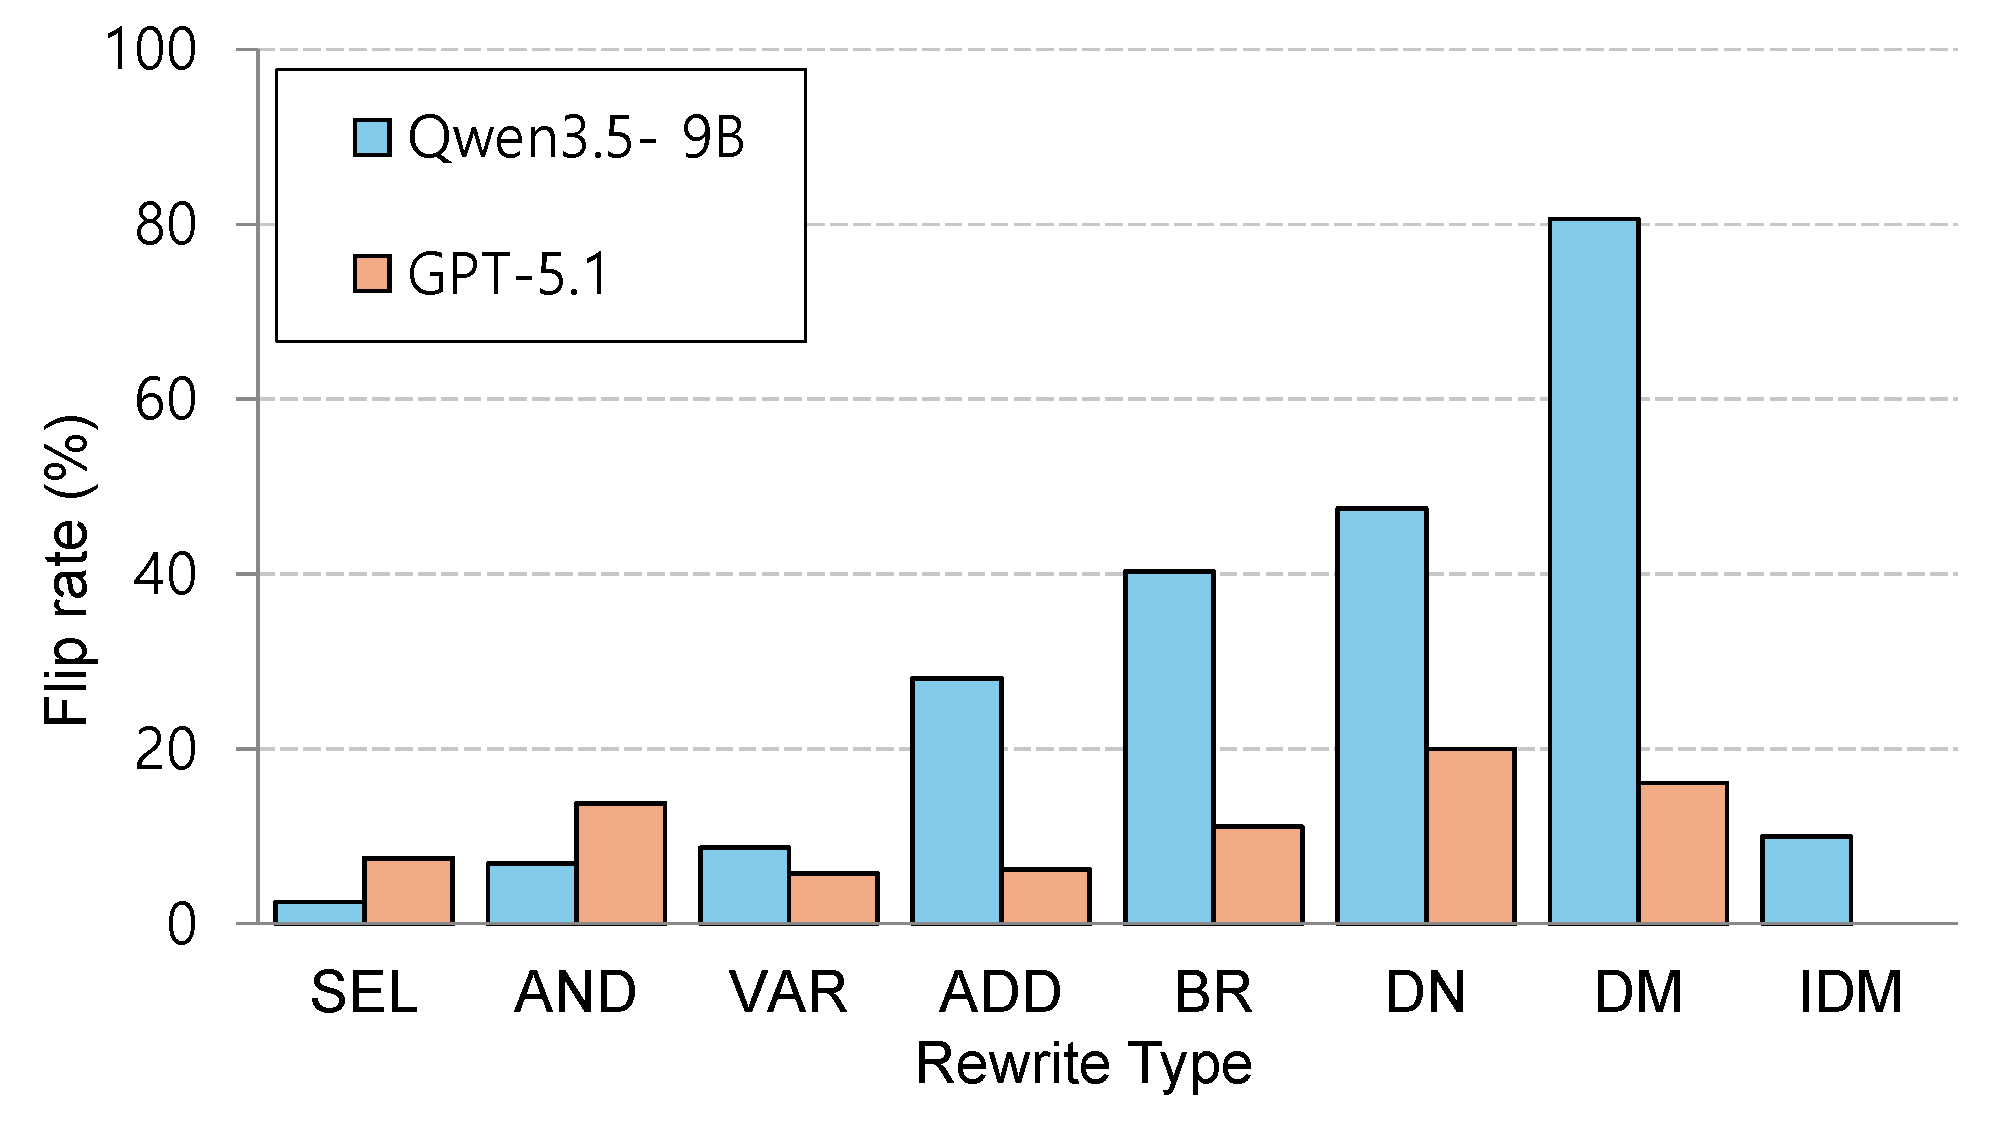
\includegraphics[width=\linewidth]{figs/instability.pdf}
\caption{LLM judge verdict flip rate by rewrite type on behavior-identical programs (temperature 0).}
\label{fig:instability}
\end{figure}

\begin{table}[t]
\centering
\caption{Overall flip rate by judge configuration; OVLA's trace check flips on none of the same rewrites.}
\label{tab:instab}
\begin{tabular}{lcc}
\toprule
Judge configuration & 9B & GPT-5.1 \\
\midrule
deterministic (temp=0) & 27.0\% & 10.6\% \\
+ sampling (temp=0.7) & 34.4\% & 12.8\% \\
+ majority vote (K=5) & 31.2\% & 13.5\% \\
\textbf{OVLA (deterministic trace)} & \textbf{0\%} & \textbf{0\%} \\
\bottomrule
\end{tabular}
\end{table}

%\textbf{The surviving design.} With every candidate eliminated, the requirements themselves indicate the shape of the solution. R1 requires that the reference be \emph{derived} from intent the user has confirmed. R2 requires that the check be deterministic over behavior, namely over traces rather than syntax. R3 requires that the check run on the device without any LLM call. A user-confirmed Timeline IR supplies the reference (R1), deterministic trace-equivalence over that IR supplies the stability (R2), and realizing the check as plain code on the hub supplies the on-device operation (R3). The representation is the Timeline IR (\S5), and the check over it is the verifier (\S6). (The judge in this motivating experiment compares natural language against code. The experiment of \S8.2 differs in that its judge is given the IR and compares the IR against the code.)
\textbf{The surviving design.}
The requirements now determine the design. R1 says that the reference must be derived from intent the user has confirmed. R2 says that the verdict must depend on behavior, not syntax. R3 says that the check must run locally without an LLM call. A user-confirmed Timeline IR satisfies the first requirement by turning the approved intent into a behavioral reference. Deterministic trace-equivalence over that IR satisfies the second by comparing action traces rather than code text. Implementing the check as ordinary verifier code on the hub satisfies the third. The representation is the Timeline IR (\S5), and the deterministic check over it is the verifier (\S6). The judge experiment above compares natural language against code; the later judge comparison in \S8.2 is different because the judge is given the IR and asked to compare IR against code.

\begin{figure*}[t]
\centering

\includegraphics[width=\textwidth]{figs/system.pdf}
\caption{OVLA system overview. ①{--}⑤ generation, ⑥{--}⑦ verification; the dashed arrow is the counterexample-guided repair loop.}
\label{fig:arch}
\end{figure*}

\section{System Overview}

%\textbf{Target platform.} OVLA realizes this design on the edge hub of a commercial IoT platform whose execution DSL is JoI. A JoI script follows the \texttt{cron}/\texttt{period}/\texttt{code} structure sketched in \S1 and implements its behavior directly with persistent variables and conditions. This DSL is the target of lowering.
OVLA implements the design of \S3 as a two-phase pipeline. In the authoring phase, the system derives a Timeline IR from the user's command, renders that IR for confirmation, and lowers the confirmed IR to executable code. In the verification phase, the system checks the generated code against the confirmed IR before deployment. The central boundary is fixed throughout the pipeline: the LLM may propose candidate artifacts, but every artifact that can affect deployment is checked by deterministic code.

%OVLA is organized around a single principle. The LLM is used only for \emph{generation}, namely proposing the IR and lowering it to JoI code, while the feasibility gate, the Rendering shown for approval, and the verifier are deterministic and make no LLM call. Figure~\ref{fig:arch} shows the full pipeline in two phases. The first phase covers authoring, so it interleaves LLM generation steps with two of the deterministic gates. The second phase is verification and runs entirely LLM-free.
\textbf{Execution target.} We instantiate OVLA on the edge hub of a commercial IoT platform whose execution DSL is JoI. A JoI automation consists of a start schedule (\texttt{cron}), a re-execution interval (\texttt{period}), and a script body (\texttt{code}). When \texttt{period} is positive, the body is executed on each tick, and temporal behavior such as edge detection, sustained conditions, and counting must be implemented with persistent variables and ordinary conditionals. JoI is therefore the executable artifact produced by lowering, and it is the artifact checked by the verifier.

Figure~\ref{fig:arch} shows the complete pipeline. The first phase is authoring: it includes LLM-based generation steps, but it also includes deterministic gates before the user approves the reference. The second phase is verification: it takes the approved IR and the generated JoI code as inputs and runs without any LLM call.

%\textbf{Phase 1: Authoring (LLM generation with deterministic gates).} ① Semantic parsing (intent analysis, device mapping, tool mapping) processes the user's natural-language command. It interprets what the user intends and maps the request onto the devices and tools available on the platform. ② From its output a \textbf{Timeline IR} is extracted. The \textbf{feasibility gate} (\S5) deterministically rejects IRs whose structure violates the IR grammar, for example a nested loop that JoI cannot realize, and the surviving IR is rendered in plain language by the deterministic \textbf{Rendering}. ③ The rendered text is shown to the user, and ④ on confirmation the Timeline IR is fixed as the reference. ⑤ The confirmed IR is \textbf{lowered} to JoI code.
\textbf{Phase 1: Authoring (LLM generation with deterministic gates).} ① OVLA first analyzes the user's natural-language command. This analysis identifies the temporal and behavioral slots that the automation must express, such as the start time, repetition period, trigger or condition, delay or sustain duration, and target action. It also maps the command onto the connected device list, selecting the relevant devices and the services that those devices must expose for the automation to be executable. ② OVLA then extracts a candidate \textbf{Timeline IR} from this analysis. The word ``candidate'' matters: before user confirmation, the IR is only the system's proposed interpretation of the command. Before any code is generated, the deterministic \textbf{feasibility gate} (\S5) checks whether this IR belongs to the supported IR grammar. It rejects structures that cannot be realized by the target execution model, such as nested cycles or misplaced branches. ③ If the IR passes this gate, OVLA renders it into the deterministic \textbf{Rendered IR} shown in Figure~\ref{fig:arch}. The Rendered IR is a plain-language view of the IR, not a new natural-language command. ④ The user reviews this Rendered IR. Once the user confirms it, the Timeline IR is fixed as the reference specification for the automation. ⑤ Only after this reference is fixed does OVLA lower the IR to JoI code.

%\textbf{Phase 2: Verification (deterministic, LLM-free).} ⑥ The verifier checks the generated JoI against the confirmed Timeline IR, which enters as the behavioral reference (the reference arrow in Figure~\ref{fig:arch}). A static check first validates the syntax of the generated JoI. The behavioral check then derives an FSM from the IR, synthesizes boundary \textbf{events} (\S6), and runs the IR simulator and the JoI simulator on the same events to compare \textbf{trace-equivalence}. ⑦ The final verdict is either deployment on a pass or a \textbf{fail-closed rejection} when repair is exhausted. On a mismatch, control returns to lowering (⑤) with a \textbf{counterexample}, and only the JoI is regenerated (dashed arrow); the IR is the approved reference and remains fixed.
\textbf{Phase 2: Verification (deterministic, LLM-free).} ⑥ The verifier receives two artifacts: the confirmed Timeline IR and the generated JoI code. The confirmed IR is the behavioral reference. The verifier first performs a static syntax check on the JoI code. The behavioral check then follows the lower half of Figure~\ref{fig:arch}. From the confirmed IR, OVLA derives an FSM that makes the enabled obligations and their reachable states explicit. The \textbf{Event Synthesis} stage generates boundary events from this FSM (\S6). The same synthesized event set is fed into two deterministic simulators: \textbf{IR-Sim}, which executes the confirmed IR, and \textbf{JoI-Sim}, which executes the generated JoI code. Their action traces are passed to the \textbf{Trace-Equivalence} stage, which decides whether the code matches the approved IR under the observation model of \S6. ⑦ A passing program is deployed. A failing program is not deployed directly. Instead, the verifier returns a \textbf{counterexample} to the lowering stage, and only the JoI code is regenerated. The confirmed IR is not changed during repair; it remains the user-approved reference. If repair is exhausted, OVLA rejects the automation fail-closed.

%\textbf{Three checks, three places.} The three checks operate at different points on different artifacts. The \textbf{feasibility gate} is a structural check on the \emph{IR} as a typed tree, immediately after IR extraction and before lowering (\S5). The \textbf{static syntax check} inspects the \emph{generated JoI code} after lowering. The \textbf{behavioral trace-equivalence check} compares the IR and the code (\S6). The behavioral check is the core of the verifier, and the other two are the gates that support it.
\textbf{Three checks, three places.} OVLA uses three deterministic checks, each on a different artifact. The \textbf{feasibility gate} checks the structure of the \emph{IR} as a typed tree, immediately after IR extraction and before lowering (\S5). The \textbf{static syntax check} checks the \emph{generated JoI code}, after lowering and before simulation. The \textbf{behavioral trace-equivalence check} compares the behavior of the confirmed IR and the generated JoI code (\S6). These checks are not interchangeable. The behavioral check is the core deployment gate, while the feasibility and syntax checks prevent malformed artifacts from reaching that gate.

%\textbf{Roles of the IR.} A single Timeline IR plays four roles. It is the artifact the user approves through its plain-language surface, and it is the verification reference. These two roles are the design properties of \S5. It further serves as a generation scaffold for lowering and as a structural signature that routes lowering exemplars (\S7). The upstream semantic parsing (intent analysis, device/tool mapping) is inherited platform infrastructure and not a contribution of this paper.
\textbf{Roles of the IR.} A single Timeline IR plays four roles in OVLA. First, it is the artifact exposed to the user through deterministic Rendering. Second, after confirmation, it is the behavioral reference used by the verifier. Third, it serves as the scaffold from which the system lowers JoI code. Fourth, its structural signature is used to route lowering exemplars (\S7). OVLA uses semantic analysis and device/service mapping as upstream stages, but the contribution of this paper begins with how the confirmed IR is rendered, fixed as a reference, lowered, and verified.

\begin{figure*}[t]
\centering
\begin{minipage}[t]{0.42\textwidth}
\centering
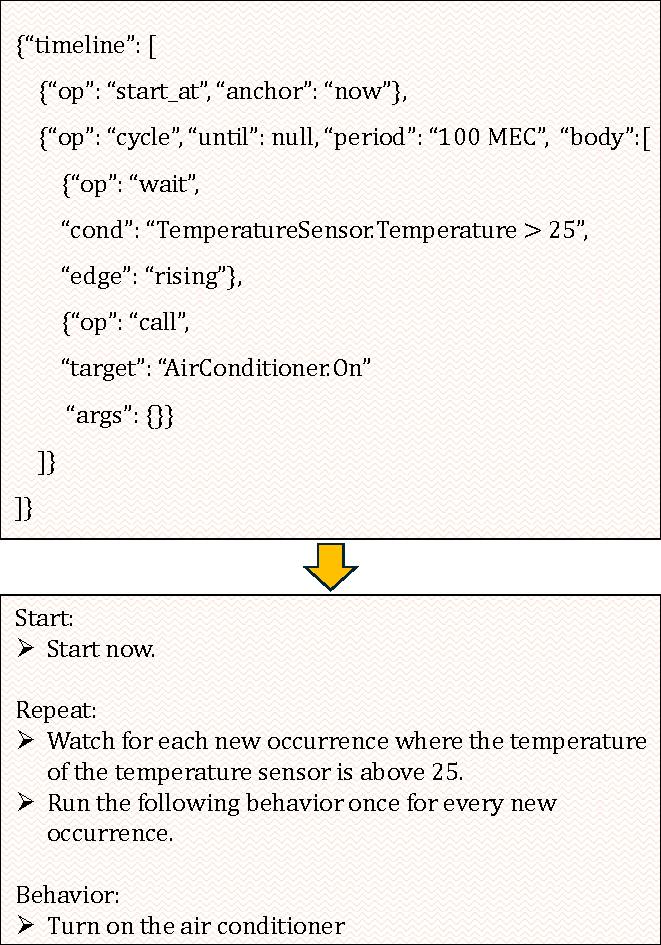
\includegraphics[width=\linewidth]{figs/Rendering1.pdf}\par
\small (a) Recurring edge trigger
\end{minipage}\hspace{0.04\textwidth}%
\begin{minipage}[t]{0.42\textwidth}
\centering
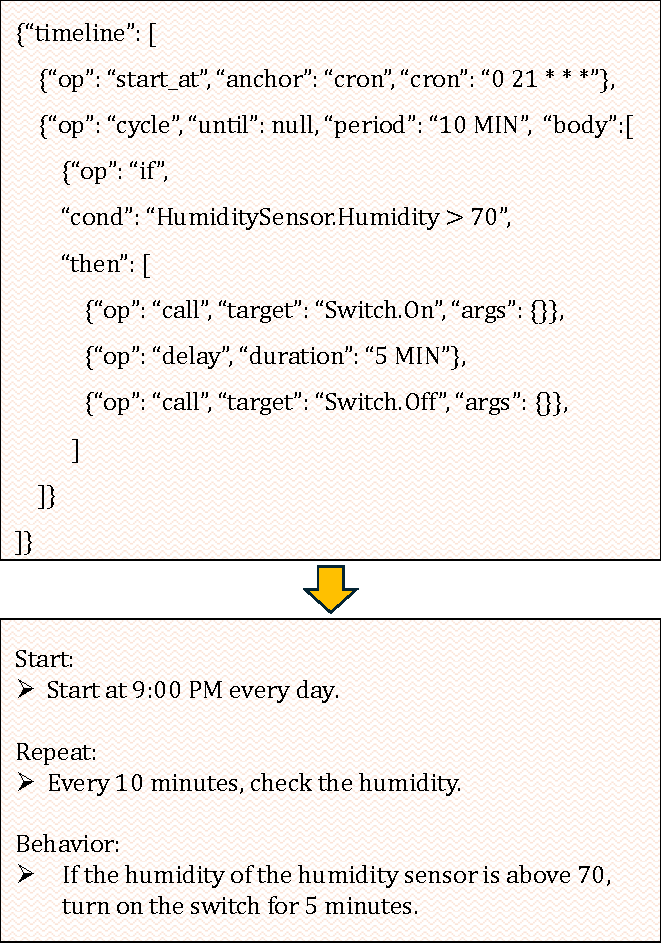
\includegraphics[width=\linewidth]{figs/Rendering2.pdf}\par
\small (b) Scheduled periodic check with branch and delay
\end{minipage}
\caption{Two Timeline IRs and their deterministic plain-language Renderings.}
\label{fig:ir}
\end{figure*}

\section{Timeline IR}

Timeline IR is designed to provide two properties at once. First, it is rendered to plain language deterministically (without an LLM) so the user can approve it. Second, it is a machine-checkable behavioral reference. NL→IR is an LLM stage, but IR→Rendering is deterministic, so the text the user sees reflects the IR exactly. The Rendering cannot introduce content the IR does not contain, and what is displayed is what is checked.

\textbf{Closed control dimensions and primitive ops.} Both properties follow from how the IR represents behavior. The dimensions a reactive-temporal command controls are closed and enumerable: start and schedule (\texttt{start\_at}), period (\texttt{cycle.period}), triggers and conditions (\texttt{wait}'s cond and edge, \texttt{if}'s cond), actions and their arguments (\texttt{call}), sustain and delay (\texttt{wait.for}, \texttt{delay}), and state and counting (persistent variables, \texttt{cycle.count}, \texttt{break}). Timeline IR assigns one primitive op to each dimension and encodes the slots the command names directly on a timeline. This canonical, minimal form yields both properties at once. (a) The deterministic Rendering puts these slots into plain language without adding information, so approving an IR is a closed judgment over the finite slots the command named, not the authoring of an arbitrary formal property. (b) The same representation doubles as a machine-checkable behavioral reference over the same closed dimensions. The closed op set is exactly what the grammar G below ranges over.

\textbf{Finite-state view.} The IR views reactive behavior as a finite set of obligations, that is, scheduled checks, waits, and actions to be discharged on the timeline. It admits no recursion and no unbounded loops, only bounded timers, counters, and finite control. The IR is not a timed-automaton model-checking target. It is simply a finite view that makes the objects of checking enumerable.

\textbf{Typed tree and dependency grammar G.} The IR is a typed tree, and a dependency grammar G fixes which structures are legal: exactly one \texttt{start\_at} (and at most one top-level cron), no \texttt{cycle} inside \texttt{cycle.body} (no nesting), \texttt{then}/\texttt{else} only as children of \texttt{if}, \texttt{break} only inside a \texttt{cycle}, and \texttt{cycle} requires a period (\texttt{until} is optional; when absent, the cycle repeats within the verifier's bounded checking horizon, \S6). Membership \texttt{IR∈L(G)} is deterministically decidable. The same single pass over the typed tree also yields the IR's structural class τ(IR), the combination of grammar rules the IR instantiates, which \S7 uses to route lowering exemplars.

\textbf{Feasibility gate.} This membership test is the feasibility gate of \S4. It rejects structurally impossible IRs (nested cycles, double cron, misplaced then/else, break outside a cycle) immediately after IR extraction. Its grammar-membership decision holds by construction and is therefore not an empirical component of the evaluation. The guarantee, however, rests on the assumption that the extractor \emph{transcribes} the user's words literally. If the LLM silently flattens an illegal structure into a legal one, the resulting IR passes G with the wrong meaning, and that semantic mismatch is left for user confirmation to catch. The extractor is therefore designed to transcribe, not to correct.

The operators are \texttt{start\_at}, \texttt{wait} (cond, edge, for), \texttt{delay} (duration), \texttt{read}, \texttt{call}, \texttt{if} (then/else), \texttt{cycle} (period, count, until, body), and \texttt{break}. Figure~\ref{fig:ir} shows two examples, each pairing an IR with its Rendering. (a) is the temperature example of \S1: ``whenever the temperature rises above 25°C'' is encoded as \texttt{wait(Temperature > 25, edge: rising)} inside a \texttt{cycle}, and the Rendering surfaces the \texttt{edge: rising} slot as ``each new occurrence'' and the \texttt{call} as ``Turn on the air conditioner.'' (b) is a schedule-driven automation: the \texttt{start\_at} cron becomes ``Start at 9:00 PM every day,'' \texttt{cycle.period} becomes ``Every 10 minutes,'' and the \texttt{if}-\texttt{call}-\texttt{delay}-\texttt{call} sequence becomes one conditional behavior sentence. Even the empty \texttt{else} branch is rendered explicitly as ``Otherwise, do nothing,'' because the Rendering neither drops nor adds slots (\S8.3).

\section{Verifier}

\subsection{Observation Model: Transition-Boundary Conformance}

The gate decides a single question: does the generated JoI code \emph{exhibit the same behavior} as the approved IR? As \S2 observed, the execution DSL has no primitives for the IR's control dimensions, so the LLM realizes each IR behavior as an idiom: ``sustained for N minutes'' becomes a counter incremented on each poll tick that fires at a threshold; ``edge (whenever)'' becomes a triggered flag set on firing and reset when the condition clears (or a prev/curr comparison); ``every N minutes'' becomes periodic re-execution of the body. One IR behavior thus appears as several valid idioms and as countless near-misses one tick or one comparison off (Figure~\ref{fig:idiom}), and this idiom-realization point is exactly where bugs enter. Equivalence must therefore be decided on behavior (traces), not on syntax.

Deciding on behavior is tractable because reactive-temporal behavior changes only at a finite set of candidate points. The only candidates at which the behavior can change are guard thresholds, condition edges, time landmarks (delay, duration, period, cron), and internal state transitions. These four axes partition the input space into finitely many cells, and within each cell the behavior is constant. Because the IR admits only bounded control, with no recursion or unbounded loops, the number of cells within a bounded horizon is finite, and one representative input per cell exercises the entire cell under this abstraction. The verifier sets the horizon to one week, because time-of-day and day-of-week schedules recur within a week, so the horizon covers one full period of every such schedule. Calendar fields of a cron (day-of-month, month) only select when that weekly pattern is active and carry no further behavioral semantics, so they are checked statically: the IR's and the code's calendar fields must denote the same set, and within any window they select, behavior recurs at the week granularity the simulation covers. We take this as the observation model, \textbf{transition-boundary conformance}: two programs behave the same if their action traces agree, within a tolerance, at the boundaries where behavior can change (threshold crossings, condition edges, timer expirations, next-cycle restarts), over the fixed bounded horizon. This is an equivalence judgment focused on boundaries, not an equivalence proof over the whole input space. Restricting the judgment to boundaries is what lets the \textbf{bounded trace-equiva\-lence} check run deterministically, solver-free, and on-device. The verifier is therefore a deployment-time filter, not a replacement for heavyweight formal methods. The internal-state axis of the abstraction cannot be dropped: implementation (b) of Figure~\ref{fig:idiom}, for example, fires or stays silent depending on a flag that sensor values alone do not determine.

\subsection{Boundary Event Synthesis}

The core technique deterministically derives an FSM from the IR, without any LLM call, and synthesizes representative events at the IR's decision points. Each op (\texttt{call}, \texttt{wait}, \texttt{delay}, \texttt{read}, \texttt{if}, \texttt{cycle}, \texttt{break}) becomes an obligation. Sequencing between ops imposes order, branches contribute guards, and \texttt{cycle} adds an obligation to re-arm for the next iteration.

A flat list of ops would not suffice, because a boundary is meaningful only in the state where its op is enabled: after the preceding waits have discharged, on the branch its guard selects, and in the iteration the cycle has reached. The FSM makes these states explicit. Each representative event is therefore scheduled at a time when its boundary is actually reachable, and is held at the boundary value. Within a cell, the exact value crossed is irrelevant (\S6.1). What matters is the timing of the crossing. When a divergence is found, it is attributed back to the obligation that owns it, and this attribution is the counterexample that the repair loop of \S4 consumes.

The synthesis is IR-based, not surface-syntax-based. It tracks read→sensor flows and seeds both ends of a value domain so that scale and offset errors surface. The IR's arithmetic helpers (\texttt{abs}, \texttt{min}, \texttt{max}) have no JoI counterpart, so the lowering unrolls them into conditional clamping code; the synthesizer therefore seeds the internal boundaries of those unrollings as well, where an inverted clamp would otherwise pass unnoticed. It skips read-modify-write accumulators and covers second-edge cases where a condition clears and later holds again. The same synthesized event set is fed to the IR simulator and the JoI simulator, so the two are compared on identical inputs.

\subsection{Trace-Equivalence and Omission Detection}

The IR simulator and the JoI simulator are run on the same events. The resulting action traces are grouped and deduplicated within a ±tolerance window (max 500ms, 10\%) and compared order-preserving. This comparison catches commission (actions that must not happen) and omission (required actions that are missing) at once, because \emph{silence} is part of a trace: an empty interval in the IR trace is an oracle saying ``nothing happens here.'' This works because the IR specifies the whole behavior rather than selected properties. Partial properties or LTL formulas do not pin down silence and therefore cannot catch omissions. For example, code that mistranslates ``check every 15 minutes'' into immediate reaction diverges from the IR in firing rate and timing on the IR's sustained-boundary scenarios (IR sparse or silent, JoI over-firing) and is flagged.

\subsection{What the Verdict Guarantees}

The verdict is deterministic and LLM-free. \textbf{T1 (determinism)}: the same (IR, code) pair always yields the same verdict. \textbf{T2 (rejection-soundness)}: when the checker flags, the flag is a real behavioral divergence under the defined observation model. We do not claim ``pass ⇒ correct.'' The trusted computing base is the two simulators, the tolerance, and the equivalence relation; the LLM is excluded. Soundness is supported by reduction to simulator fidelity rather than by proof, and the adequacy of the check is established empirically with mutation testing derived from the IR constructs and coverage measured on both the specification and implementation sides (\S8.2). Surviving mutants are characterized individually.

\subsection{Limits of the Check}

The observation model leaves explicit residual limits. Schedules are fully covered by the one-week horizon and the static calendar check (\S6.1), but behaviors whose own durations exceed a week, such as a month-long sustain, are not exercised to completion. Variable-to-variable arithmetic without a threshold (e.g., \texttt{notify(\$t1-\$t2)}) offers no boundary to target, so only generic seeds apply: sign and structure bugs are caught, but value-specific bugs that fire only under particular value relations can be missed. These are limits on which divergences the synthesized events exercise, not a source of false passes, because both simulators share the same values.

\section{Implementation}

OVLA's deterministic core is pure Python with no external dependencies. The two simulators (about 3.7K lines), the verifier (1.1K), the Rendering (0.7K), and the feasibility gate (0.1K) total roughly 5.7K lines of deterministic code, with no solver and no model call. Generation runs on off-the-shelf 4-bit-quantized models of at most 9B parameters, without fine-tuning (\S8 Setup). Generation is decomposed into the stages of \S4 (intent analysis, device and tool mapping, IR extraction, lowering), and the verifier's guarantee is independent of which generator produced the code.

\textbf{Structure-based example routing.} The lowering prompt does not carry few-shot examples for every idiom family. Because the feasibility pass (\S5) already computes the IR's structural class τ(IR), the prompt injects only the K examples whose structure matches the new IR, which keeps the prompt short on a small on-device model. The example bank maintains itself: every (IR, JoI) pair that passes the verifier is appended under its signature, so a pair that once failed and was repaired contributes its corrected lowering to future requests of the same class. Routing shapes only the generator's prompt; the accept/reject verdict remains the deterministic check of \S6. We do not ablate the effect of routing in this submission, so we describe the mechanism without quantitative claims about generation improvement.

\section{Evaluation}

The goal of the evaluation is not an accuracy contest but to establish, component by component, that each link of the workflow holds. The central result is system safety: silent IR-code divergence drops to zero (\S8.1).

\textbf{Setup.} \emph{Hardware}: the primary edge device is a Mac mini M4 (16GB); accuracy results are obtained on GPU servers. \emph{Models}: generation uses Qwen3.5-9B, with Qwen3-8B and Gemma-4-E4B as additional generators (Table~\ref{tab:models}); all are 4-bit quantized without fine-tuning (AWQ on the GPU servers, MLX on the M4). Safety results are backend-independent: on-device cost is measured on the M4, and zero silent divergence is invariant across backends and generators. \emph{Dataset}: 382 automations in 24 categories. The commands were written to cover the reactive idiom families (triggers, edges, sustains, periodics, sequences, branches, counting) over devices the platform's service catalog supports, not curated to fit OVLA's grammar, and the ground-truth IRs passed an independent value-level audit that fixed the set at 382. \emph{Baseline}: the main comparison is the verification alternative, an LLM judge; for every judge we state, with the result it accompanies, the input artifact (request, IR, or code), temperature, and voting configuration. \emph{Metrics}: safety (silently divergent code deployed), detection (detection/FP/FN), faithfulness (surface rate), and on-device cost (latency distribution, memory, power).

\subsection{RQ1: System Safety}

Does OVLA prevent deployed code from silently diverging from the \emph{displayed IR}? We measure the gate as a paired ablation: both arms share the same lowering candidates, and the gated arm verifies each candidate, deploys it if it passes, and otherwise enters the diagnose-and-repair loop (at most two attempts, then fail-closed rejection). Without the gate, 33 of 382 automations (8.6\%) would deploy while silently diverging from the IR displayed for approval. The gate reduces this to zero: of the 33, 11 are repaired and 22 are rejected fail-closed. The fraction of requests that end deployed and correct rises from 91.36\% to 94.24\% (349→360 of 382). What counts as divergence here is the verifier's verdict; that this verdict tracks real behavioral faults is established independently in \S8.2 against injected mutations and naturally occurring logic faults. We additionally audited all 33 flagged lowerings by hand: 31 are genuine behavioral divergences (sustain mistimings, inverted logic, counter misuse, structural duplication), and 2 are fail-closed rejections of code outside the simulatable subset (unparseable statements); none is a misjudged correct program. These numbers concern divergence from the \emph{displayed} IR (the confirmed-IR assumption), not whether the IR matched the user's true intent (Layer A; \S9).

\emph{Repair is not the safety evidence.} The safety claim lies in fail-closed: divergent code is repaired or rejected, and never deployed. Because the gate is deterministic, this property does not depend on generation stochasticity: whichever candidates the model produces, a candidate divergent under the bounded observation model cannot deploy silently. The hard core of rejects concentrates in sustain timing, read-modify-write, and multi-step automations, showing that fail-closed is not ``rejecting everything hard.''

\emph{Across generation models.} The gate's behavior is consistent across the three tested generators. Replacing the 9B generator with weaker models produces up to 1.8$\times$ more divergent lowerings, and the error rate is not monotone in model size, yet none deploys silently: silent-wrong is 0 for all three generators (Table~\ref{tab:models}).

\begin{table}[t]
\centering
\caption{The gate across generation models (382 automations, confirmed IR).}
\label{tab:models}
\small
\begin{tabular}{lrrrrr}
\toprule
Generator (4-bit, no FT) & \multicolumn{1}{c}{Silent-wrong} & \multicolumn{1}{c}{Silent-wrong} & Rep. & Rej. & Deployed \\
 & \multicolumn{1}{c}{w/o gate} & \multicolumn{1}{c}{w/ gate} & & & correct \\
\midrule
Qwen3.5-9B  & 33 (8.6\%)  & \textbf{0} & 11 & 22 & 360 (94.2\%) \\
Qwen3-8B    & 61 (16.0\%) & \textbf{0} & 11 & 50 & 332 (86.9\%) \\
Gemma-4-E4B & 55 (14.4\%) & \textbf{0} & 16 & 39 & 343 (89.8\%) \\
\bottomrule
\end{tabular}
\end{table}

\subsection{RQ2: Verifier Detection}

Does the verifier catch wrong code? We look at two layers, real bugs and synthetic bugs. The real layer comes from the 382-automation pipeline of \S8.1: all 33 real LLM lowering outputs that diverged from the displayed IR were flagged, and none escaped silently. RQ1 measured these cases as a deployment outcome; here the same 33 cases are restated as detector verdicts, not as additional evidence.

\textbf{Mutation (stress coverage).} We then stress the mechanism with exhaustive construct-derived mutation (Table~\ref{tab:mutation}). Twelve operators generate every first-order mutant at every applicable site (331 seeds, 1,675 generated, 108 equivalents excluded against all scenarios), and 1,556 of 1,567 genuine mutants are caught (99.3\%). The adequacy of the synthesized scenario suite is measured as two-sided coverage (Table~\ref{tab:coverage}): the spec side exercises 97.4\% of IR-FSM obligations (342/351), with all 9 uncovered ones being unsynthesizable else-branch guards (7 variable-to-variable comparisons, 2 arithmetic); the implementation side exercises 96.8\% of generated-JoI branches (670/692).

The 11 survivors are characterized exhaustively rather than bucketed: 8 are \texttt{>=}→\texttt{>} comparator mutants on sustain tick-counters whose 1-tick difference lies below the tolerance (max 500ms, 10\%; by design); 1 is a dropped duplicate call in a two-room fan-out (\texttt{call\_drop}); and 2 sit in a single arithmetic read-modify-write automation that boundary seeding cannot reach (one \texttt{call\_drop}, one \texttt{cmp\_direction}), the read-modify-write seeding exclusion of \S6.2.

We separate three claims: ① it catches real lowering bugs (33/33, \S8.1); ② a one-construct perturbation of correct code is caught (the mutation kill rate); ③ silent mismatches in the 382 pipeline are zero (\S8.1). The mutation operators are not hand-picked: they are derived from the IR constructs, and every construct is reached by at least one operator. Mutation alone, being keyed to the same construct set the verifier checks, measures the reach of the mechanism rather than external validity; external validity rests on the real-fault layer above, and the implementation-side coverage shows the synthesized scenarios exercise the generated code, not only the spec. The soundness statement is rejection-sound, bounded-incomplete, and auditable (not ``pass ⇒ correct'').

\begin{table}[t]
\centering
\caption{Construct-derived mutation results (331 seeds, 12 operators).}
\label{tab:mutation}
\small
\setlength{\tabcolsep}{4.5pt}
\begin{tabular}{lrrrr}
\toprule
Operator & Gen. & Equiv. & Genuine & Caught (\%) \\
\midrule
arg\_numeric    & 146 & 1  & 145 & 145 (100) \\
enum\_flip      & 111 & 2  & 109 & 109 (100) \\
call\_drop      & 439 & 4  & 435 & 433 (99.5) \\
call\_add       & 202 & 3  & 199 & 199 (100) \\
tick\_scale     & 57  & 0  & 57  & 57 (100) \\
guard\_polarity & 198 & 0  & 198 & 198 (100) \\
comparator      & 163 & 38 & 125 & 117 (93.6) \\
assign\_init    & 71  & 13 & 58  & 58 (100) \\
cmp\_direction  & 163 & 30 & 133 & 132 (99.2) \\
arith\_op       & 42  & 12 & 30  & 30 (100) \\
break\_drop     & 29  & 5  & 24  & 24 (100) \\
wait\_drop      & 54  & 0  & 54  & 54 (100) \\
\midrule
Total           & 1,675 & 108 & 1,567 & 1,556 (99.3) \\
\bottomrule
\end{tabular}
\end{table}

\begin{table}[t]
\centering
\caption{Two-sided coverage of the scenario suite (spec: IR-FSM obligations; impl: generated JoI branches).}
\label{tab:coverage}
\small
\begin{tabular}{lrrr}
\toprule
Obligation & Total & Covered & (\%) \\
\midrule
\texttt{if}: then branch            & 166 & 166 & 100 \\
\texttt{if}: else branch            & 37  & 28  & 75.7 \\
\texttt{wait} (edge/sustain/re-arm) & 122 & 122 & 100 \\
arithmetic expr boundary (lo/hi)    & 26  & 26  & 100 \\
\midrule
Spec total (IR-FSM)                 & 351 & 342 & 97.4 \\
Impl: generated JoI branches        & 692 & 670 & 96.8 \\
\bottomrule
\end{tabular}
\end{table}

\textbf{vs.\ an LLM judge.} We compare the same IR↔code judgment against an LLM judge in the cloud-judge style of ChatIoT's Evaluator~\cite{chatiot}. The judge is given the IR, the JoI grammar, and the same equivalence definition including the timing tolerance, at temperature 0 with a single query; ground truth is objective (a verifier-clean lowering is correct, a non-trace-equivalent mutant of it is wrong). On 346 such programs (277 faulty, 69 correct), the 9B judge misses 36 of the faulty programs (recall 0.87) and falsely rejects 17 of the 69 correct ones; a strong cloud judge (GPT-5.1) still misses 16 (recall 0.94) and falsely rejects 14. On 30 behaviorally-correct idiom variants of the same intents (multi-GT), the 9B judge over-rejects 2 and the cloud judge 1, while the trace check passes all 30 idiom-invariantly. (This setting gives the judge the IR; it is a different experiment from the NO-IR motivating experiment of \S3.)

\subsection{RQ3: Rendering Faithfulness}

RQ3 checks one narrow prerequisite: \emph{does the deterministic Rendering expose every behavior-relevant IR difference in plain language?} We do not evaluate whether users approve the right IR (no human-subjects study; Layer A is \S9). We evaluate whether the approval surface is faithful, that is, whether the IR fields the gate consumes show up in the displayed text.

The claim is precise: the renderer exposes the IR fields that the checker and the lowerer consume, so faults in the IR-to-code relation are visible in the displayed text, and every behavioral difference in our test set produced a different Rendering. All 1,504 synthetic pairs across 8 fault classes surfaced as distinct text, with zero blind spots (Table~\ref{tab:faithful}). Of 57 real logic faults, 56 surfaced; the remaining one (C16\_5) is an upstream extraction defect in which the extractor leaked selector syntax into the IR, not a rendering blind spot. One pair suffices to show what surfacing looks like. In the oneshot↔wait-until class, the correct IR renders as ``If the charging state of the charger is fullyCharged, turn off the selected switch.'' while the faulty IR renders as ``Wait until the charging state of the charger is fullyCharged is true. Turn off the selected switch.'' A one-sentence difference exposes, in plain language, the same class of behavioral difference as the re-fire bug of \S1 (Figure~\ref{fig:idiom}(c)).

\begin{table}[t]
\centering
\caption{Rendering faithfulness: do behaviorally different IR pairs render differently?}
\label{tab:faithful}
\small
\begin{tabular}{lrrr}
\toprule
Fault class & n & Surfaced & Blind \\
\midrule
comparator                & 267 & 267 & 0 \\
polarity                  & 85  & 85  & 0 \\
wrong arg value           & 235 & 235 & 0 \\
wrong device              & 382 & 382 & 0 \\
timing/duration           & 74  & 74  & 0 \\
oneshot↔wait-until        & 150 & 150 & 0 \\
single↔cycle (whenever)   & 273 & 273 & 0 \\
AND-conjunct drop         & 38  & 38  & 0 \\
\midrule
Synthetic total (Part B)   & 1,504 & 1,504 & 0 \\
Real logic faults (Part A) & 57  & 56  & 1 \\
\bottomrule
\end{tabular}
\end{table}

\textbf{What does not surface.} This result does not mean every kind of error shows up in the text. (a) Device-name ambiguity: the same text can be interpreted onto different device bindings; binding is handled by the parallel precision channel. (b) Misread domain terms: a user may read the text differently, which is human behavior we do not evaluate. (c) Missing intent: what the user never said is absent from the IR and hence from the Rendering. (d) Unsupported constructs rejected before rendering. Our claim is that reactive-temporal \emph{logic} faults surface in plain language, something prior work shows is hard even to read off raw rules (TAP-Debug~\cite{tapdebug}: all 21 misreadings led to task failure).

\subsection{RQ4: On-Device Cost and Deployment}

\textbf{On-device cost.} We report latency as a distribution rather than a mean. On the M4, the verifier checks an automation in 0.97ms at the median over all 382 automations (10 repetitions each; p95 0.70s, worst 8.4s). The worst case is not structural complexity but the one class whose specification itself acts on every tick (1-second level-triggered polling over the verification horizon); it is bounded by the tick cap and remains below the local judge's own tail latency (p95 25.3s). The verifier process peaks at 54MB of memory and never touches the GPU (5.5W CPU during verification, versus 10.2W GPU during generation).

The key comparison: the LLM-free verifier costs about a millisecond and \$0; a local judge running the same 8B model on the same device takes 5.1s per check at the median (p95 25.3s, about 5{,}200$\times$), with the serving stack holding 11.6GB of memory; a cloud judge adds fees and a network dependency.

Authoring is a one-time cost of a few minutes per automation (cold 151s, warm 70--155s, dominated by the LLM stages); the deployed automation makes zero LLM calls. Efficiency numbers are reported as the precondition for on-device deployment, not as a contribution in themselves.

\begin{figure}[t]
\centering
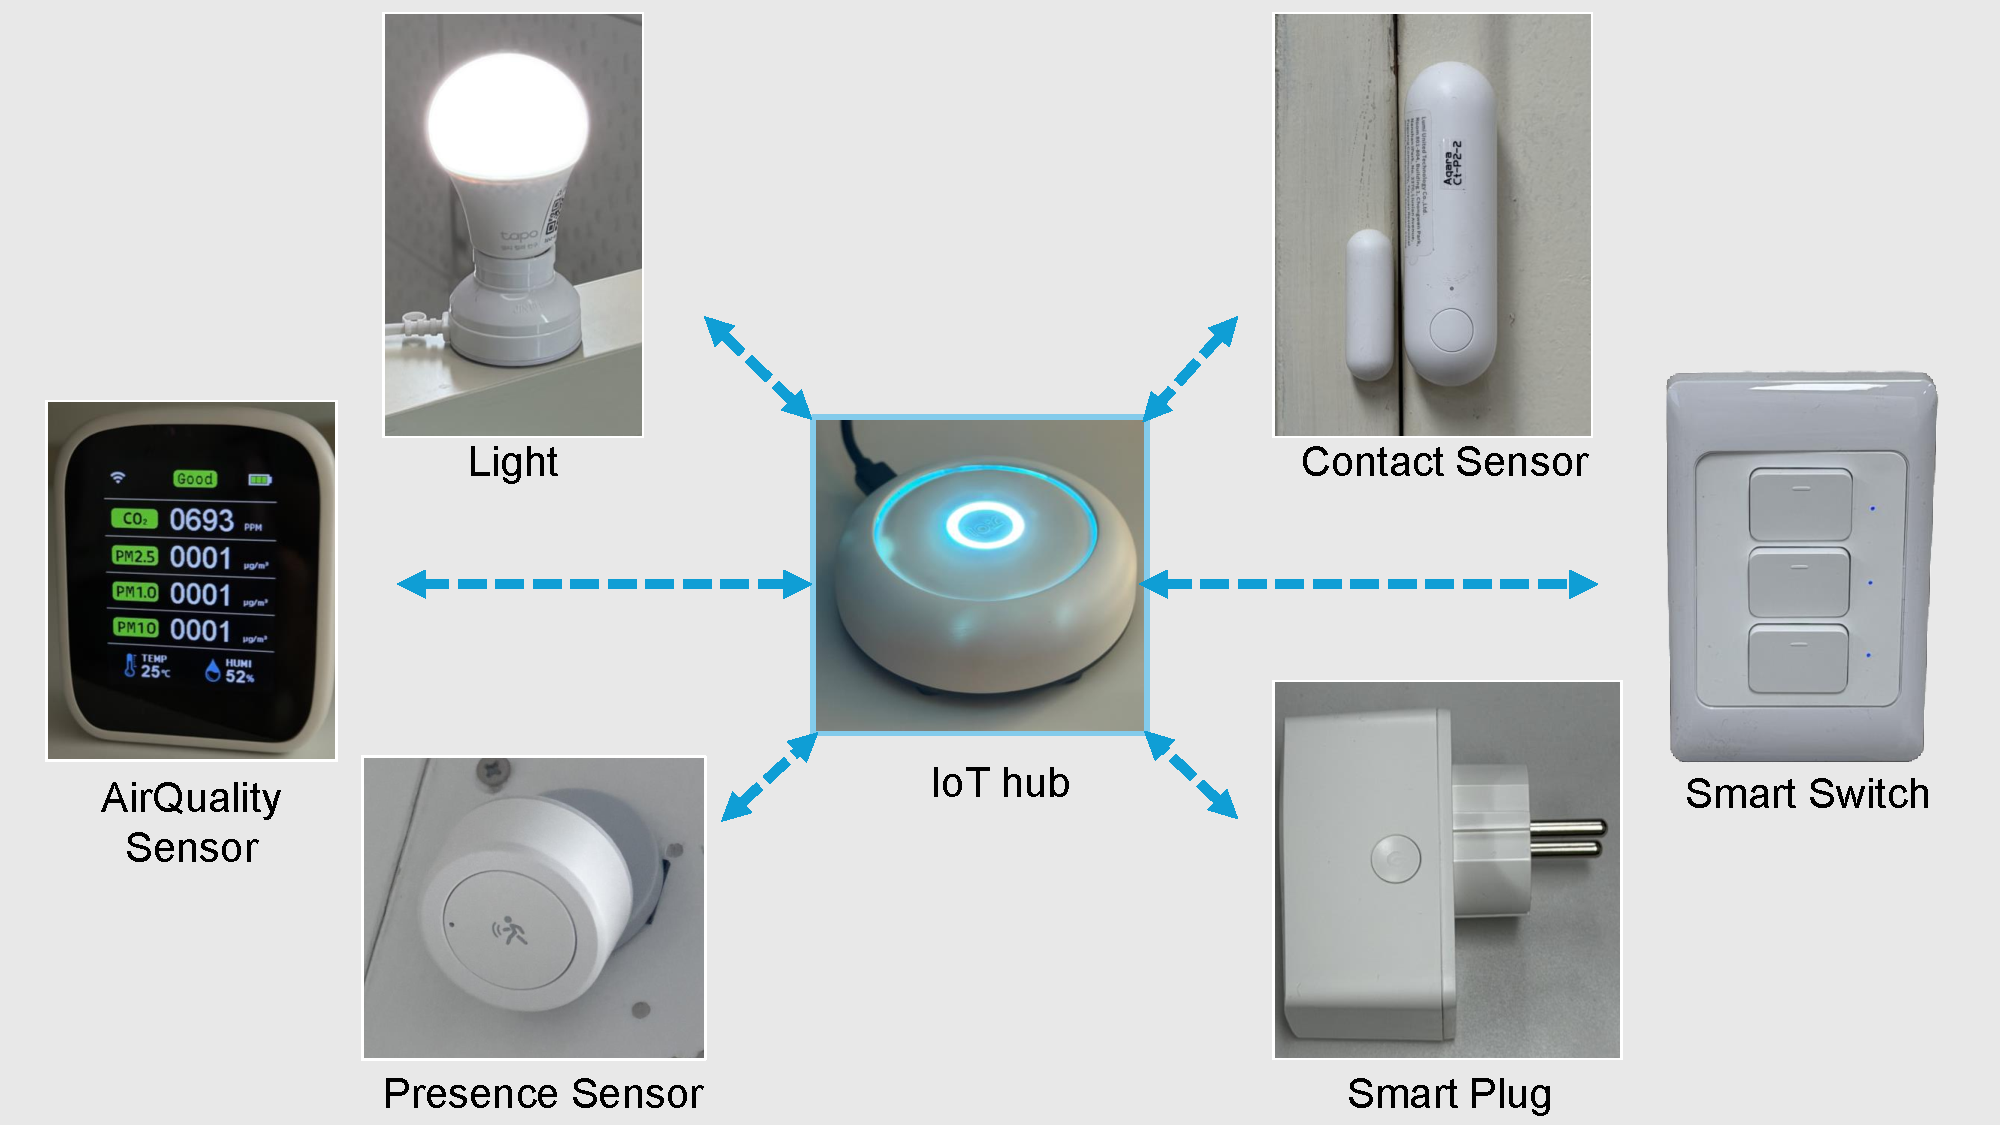
\includegraphics[width=.95\linewidth]{figs/Environment.pdf}
\caption{The physical testbed: a commercial edge hub with the sensors and actuators used in the deployment demonstration.}
\label{fig:testbed}
\end{figure}

\textbf{Deployment.} On a commercial home-automation platform (name withheld for review) with a Raspberry Pi based edge hub and physical devices (presence, contact, and air-quality sensors; plugs, lights, and a speaker; Figure~\ref{fig:testbed}), we authored six new commands live on the testbed through the full pipeline (IR extraction, confirmation, lowering, gate) and registered the gate-approved lowerings; this is an existence proof, not statistics. The representative automation, ``if no one is present in the meeting room for at least 5 minutes, turn off the TV plug,'' reproduced the sustain fault class naturally: all four ungated generations were divergent (firing after 30 or 3 seconds instead of 5 minutes), and five of six gated authoring sessions ended in fail-closed rejection before one session's repair produced a correct lowering. Figure~\ref{fig:rq4} shows the observed device behavior: without the gate the TV plug switches off 30 seconds after the room is vacated; with the gate, at 5 minutes, matching the IR-predicted trace. Across the registered automations (edge trigger, counted cycle, delay sequence, and two rising-threshold automations), every observed action sequence matched the IR-predicted trace at the platform's logging resolution (Table~\ref{tab:deploy}), including the negative obligations (a counted cycle stopping after exactly 3 announcements; no re-announcement while a crossed threshold stays high). Authoring also exercised the upstream gates: two initial wordings produced a one-shot conditional IR whose rendering revealed the misreading at confirmation, and one produced an out-of-catalog target that was rejected fail-closed at extraction validation.

\begin{table}[t]
\centering
\caption{Live-authored automations on the physical testbed: gate outcome and predicted-vs-observed behavior.}
\label{tab:deploy}
\small
\setlength{\tabcolsep}{4pt}
\begin{tabular}{llll}
\toprule
Automation & Idiom & Gate & Observed \\
\midrule
presence absent 5min → TV plug off & sustain & repaired & off at 5:00 \\
speak every 30s, 3 times only & count & pass & 3 only, stops \\
door opens → light on & edge & pass & immediate \\
light off, on after 3min & delay & pass & on at 3:00 \\
CO\textsubscript{2} rises above 900 → announce & rising & pass & on crossing only \\
temp.\ rises above 28° → switch on & rising & pass & on crossing only \\
\bottomrule
\end{tabular}
\end{table}

\begin{figure}[t]
\centering

\includegraphics[width=.92\linewidth]{figs/deployment.pdf}
\caption{The representative automation on the physical testbed: without the gate, the naturally generated buggy lowering turns the TV plug off 30 seconds after the room is vacated; the gate-repaired lowering fires at 5 minutes, matching the IR-predicted trace.}
\label{fig:rq4}
\end{figure}

\section{Limitations}

The largest limitation is that NL→IR intent correctness remains open (Layer A). A user can approve a mis-displayed IR, in which case the verifier faithfully checks against the wrong spec. We do not study human confirmation behavior in this round; we establish only that the rendering is a deterministic, faithful plain-language surface. Ethics: no human-participant data was collected (``Not applicable: no human participants'').

Beyond that, the limits are: the coverage ceiling (unsynthesizable else-branch guards: variable-to-variable comparisons and arithmetic; \S8.2); boundary-focused equivalence is not a whole-input-space guarantee; the bounded 7-day horizon; continuous arithmetic (SMT as future work); thresholdless variable-to-variable arithmetic (a coverage limit, not a soundness issue); two reads of the same service collapsing onto one device key in the selector-free IR (precision is outside this paper's scope); and generalization beyond one platform.

\section{Conclusion}

Reactive-temporal IoT automations have become easy to generate with LLMs, but the step that decides whether they are correct to deploy has been empty. OVLA confines the LLM to generation and makes the deployment gate deterministic and LLM-free: the user approves a plain-language Rendering of the IR, a deterministic checker tests the generated code against that approved IR by bounded trace-equivalence, and divergent code is repaired or rejected fail-closed. Across 382 automations, the 8.6\% that would have deployed while silently diverging from the displayed IR drops to zero, with no LLM in the verification loop, on an edge device. OVLA does not solve natural-language intent correctness, but it removes the separate silent failure mode that survives user approval.

\balance
\bibliographystyle{ACM-Reference-Format}
\bibliography{refs}
\end{document}
